\documentclass[russian,a4paper,12pt]{scrartcl}
\usepackage{babel}
\usepackage[utf8]{inputenc}
\usepackage[left=3cm,right=1cm,top=1cm,bottom=1cm]{geometry}
\usepackage{misccorr}
\usepackage{amsmath}
\usepackage{minted}
\usepackage{paralist}
\usepackage{graphicx}
\usepackage{xcolor}
\usepackage{dirtytalk}

\begin{document}
	\begin{center}
	
	\large{МИНИСТЕРСТВО ОБРАЗОВАНИЯ И НАУКИ\\ РОССИЙСКОЙ ВЕДЕРАЦИИ} \par
	\text{федеральное государственное автономное образовательное учреждение}\\ \text{высшего образования} \par
	\text{<<Санкт-Петербургский Государственный университет}\\ 
	\text{Аэрокосмического Приборостроения>>} \par
	
	\vspace{10mm}
		
	\MakeUppercase{КАФЕДРА 14} \par 
		
	\vspace{20mm}
	\begin{flushleft}
		{ОТЧЕТ}\par
		{ЗАЩИЩЕН С ОЦЕНКОЙ}\par \vspace{2mm}
		{ПРЕПОДАВАТЕЛЬ}\par
			\[
			\underset{\text{должность}}{\underline{\hspace{1cm}\text{\strut асс.}\hspace{1cm}}}
			\quad\underset{\text{подпись, дата}}{\underline{\strut\hspace{4cm}}}
			\quad\underset{\text{инициалы, фамилия}}{\underline{\hspace{1cm}\text{\strut С.В. Осмоловский}\hspace{1cm}}}
			\]
	\end{flushleft}
	\vspace{15mm}

	\textbf{ОТЧЕТ О ЛАБОРАТОРНОЙ РАБОТЕ №1}\vspace{5mm}\par{МЕХАНИЗМЫ СИНХРОНИЗАЦИИ И ВЗАИМОДЕЙСТВИЯ (IPC): МЕЖПОТОКОВАЯ СИНХРОНИЗАЦИЯ.}\par{по курсу: СИСТЕМЫ РЕАЛЬНОГО ВРЕМЕНИ} \par \par
		
	\vspace{25mm}

	\begin{flushleft}
		\text{РАБОТУ ВЫПОЛНИЛ}
		$
			\text{СТУДЕНТ ГР.} \quad
			\underline{\hspace{5mm}\text{\strut 1441}\hspace{5mm}} 
			\quad\underset{\text{подпись, дата}}{\underline{\strut \hspace{4cm}}}\quad
			\underset{\text{инициалы, фамилия}}{\underline{\hspace{5mm}\hspace{5mm}\text{\strut А.А. Протасов}\hspace{5mm}}}
		$
		\end{flushleft}
	\vspace{50mm}
	
		\text{Санкт-Петербург 2017}
	\newpage
	
	\end{center}
	\section{Постановка задачи}
	Решить одну из классических задач синхронизации в информатике: с классическим или модифицированным условием. Для решения задачи необходимо использовать определенный механизм синхронизации, предоставляемой QNX: мьютексы, семафоры, спинлоки, блокировки чтения-записи, условные переменные,  барьеры, или любой (любые) на собственное усмотрение, если в задании не указан конкретный механизм для решения. В данном случае для решения запрещается использовать способы, которые указаны в других вариантах с данной задачей.\par
	\textbf{Вариант 5}
	Задача о читателях-писателях. Приоритет писателя. 10 читателей, 5 писателей.
	\section{Пояснение}
	\textbf{Задача о читателях-писателях} — одна из важнейших задач параллельного программирования. Формулируется она так:\par
	\say{Есть область памяти, позволяющая чтение и запись. Несколько потоков имеют к ней доступ, при этом одновременно могут читать сколько угодно потоков, но писать — только один. Как обеспечить такой режим доступа?}
	\subsection{Первая задача о читателях-писателях (приоритет читателя)}
	Формулировка:\par
	\say{Пока память открыта на чтение, давать читателям беспрепятственный доступ. Писатели могут ждать сколько угодно.}
	\subsection{Вторая задача о читателях-писателях (приоритет писателя)}
	Формулировка:\par
	\say{Как только появился хоть один писатель, читателей больше не пускать. При этом читатели могут простаивать.}
	\subsection{Третья задача о читателях-писателях (честное распределение ресурсов)}
	Формулировка:\par
	\say{Не допускать простоев. Другими словами: независимо от действий других потоков, читатель или писатель должен пройти барьер за конечное время.}
	\newpage
	\section{Листинги}
	\usemintedstyle{autumn}
	\inputminted[
			frame=lines,
			framesep=2mm,
			baselinestretch=1.2,
			fontsize=\footnotesize,
			linenos
			]{c}{main.c}
	\newpage
	\section{Выводы}
		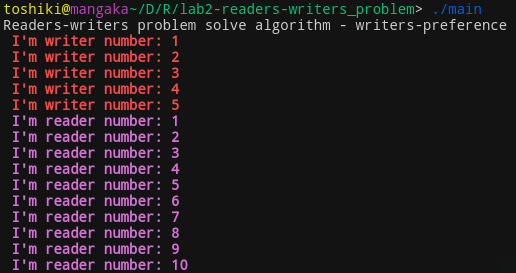
\includegraphics[scale=0.7]{Screen}
\end{document}